\documentclass[landscape,final]{baposter}

\usepackage{times}
\usepackage{calc}
\usepackage{graphicx}
\usepackage{amsmath,amssymb,amsthm}
\usepackage{relsize}
\usepackage{multirow}
\usepackage{bm}

\usepackage{graphicx}
\usepackage[pdf]{pstricks}
\usepackage{multicol}

\usepackage{pgfbaselayers}
\pgfdeclarelayer{background}
\pgfdeclarelayer{foreground}
\pgfsetlayers{background,main,foreground}

\newcommand{\captionfont}{\footnotesize}

\selectcolormodel{cmyk}

%%%%%%%%%%%%%%%%%%%%%%%%%%%%%%%%%%%%%%%%%%%%%%%%%%%%%%%%%%%%%%%%%%%%%%%%%%%%%%%%
% Multicol Settings
%%%%%%%%%%%%%%%%%%%%%%%%%%%%%%%%%%%%%%%%%%%%%%%%%%%%%%%%%%%%%%%%%%%%%%%%%%%%%%%%
\setlength{\columnsep}{0.7em}
\setlength{\columnseprule}{0mm}


%%%%%%%%%%%%%%%%%%%%%%%%%%%%%%%%%%%%%%%%%%%%%%%%%%%%%%%%%%%%%%%%%%%%%%%%%%%%%%%%
% Save space in lists. Use this after the opening of the list
%%%%%%%%%%%%%%%%%%%%%%%%%%%%%%%%%%%%%%%%%%%%%%%%%%%%%%%%%%%%%%%%%%%%%%%%%%%%%%%%
\newcommand{\compresslist}{%
\setlength{\itemsep}{1pt}%
\setlength{\parskip}{0pt}%
\setlength{\parsep}{0pt}%
}

\newtheorem{proposition}{Proposition}
\theoremstyle{definition}
\newtheorem{definition}{Definition}

\DeclareMathOperator*{\argmin}{argmin}
\DeclareMathOperator*{\argmax}{argmax}

%%%%%%%%%%%%%%%%%%%%%%%%%%%%%%%%%%%%%%%%%%%%%%%%%%%%%%%%%%%%%%%%%%%%%%%%%%%%%%
%%% Begin of Document
%%%%%%%%%%%%%%%%%%%%%%%%%%%%%%%%%%%%%%%%%%%%%%%%%%%%%%%%%%%%%%%%%%%%%%%%%%%%%%

\begin{document}

%%%%%%%%%%%%%%%%%%%%%%%%%%%%%%%%%%%%%%%%%%%%%%%%%%%%%%%%%%%%%%%%%%%%%%%%%%%%%%
%%% Here starts the poster
%%%---------------------------------------------------------------------------
%%% Format it to your taste with the options
%%%%%%%%%%%%%%%%%%%%%%%%%%%%%%%%%%%%%%%%%%%%%%%%%%%%%%%%%%%%%%%%%%%%%%%%%%%%%%
%
% Poster board dimensions will be posted here when confirmed. The typical size for poster boards in European conferences is 2 meters tall by 1 meter wide.
%
% The title of your poster should appear at the top in CAPITAL letters about 25mm high. Below the title put the author(s)' name(s) and affiliation(s). The flow of your poster should be from the top left to the bottom right. Use arrows to lead your viewer through the poster. Use color for highlighting and to make your poster more attractive. Use pictures, diagrams, cartoons, figures, etc., rather than text wherever possible. Try to state your main result in 6 lines or less, in lettering about 15mm high so that people can read the poster from a distance. The smallest text on your poster should be at least 9mm high, and the important points should be in a larger size. Use a sans-serif font (such as "cmss" in the Computer Modern family or the "Helvetica" PostScript font) to make the print easier to read from a distance.

\typeout{Poster Starts}

\background{
  \begin{tikzpicture}[remember picture,overlay]%
    \draw (current page.north west)+(-2em,-0em) node[anchor=north west] {\hspace{-2em}\includegraphics[height=1.1\textheight]{silhouettes_background}};
  \end{tikzpicture}%
}

\definecolor{LightBlue}{rgb}{0.9,0.9,0.8}
\definecolor{LightGreen}{rgb}{0.8,0.9,0.8}
\definecolor{LightGray}{rgb}{0.9,0.9,0.9}
\definecolor{DarkGray}{rgb}{0.8,0.8,0.8}
\definecolor{DarkerGray}{rgb}{0.2,0.2,0.2}
\definecolor{TelecomRed}{rgb}{0.78,0.05,0.12}

\begin{poster}
{
  columns=4,
  % Show grid to help with alignment
  grid=no,
  % Column spacing
  colspacing=1em,
  % Color style
  bgColorOne=white, % DarkGray,
  bgColorTwo=white, % LightGray,
  borderColor=LightGray,
  headerColorOne=LightGray,
  headerColorTwo=LightGray,
  headerFontColor=TelecomRed,
  boxColorOne=LightGray,
  boxColorTwo=LightGray,
  % Format of textbox
  textborder=rectangle,
  % Format of text header
  eyecatcher=yes,
  headerborder=open,
  headerheight=0.2\textheight,
  headershape=rectangle,
  headershade=plain,
  headerfont=\bf\Large\textsf, %Sans Serif
  boxshade=plain,
%  background=shade-tb,
  background=plain,
  linewidth=0pt
  }
  % Eye Catcher
  {
  	
\includegraphics[height=3.8cm]{logoTPT}
  }
  % Title
  {\sf %Sans Serif
  \huge
MULTIPITCH\, ESTIMATION\, USING\, A\, PCLA-BASED\\ \vspace{3mm}
MODEL:\, IMPACT\, OF\, PARTIAL\, USER\, ANNOTATION}
  % Authors
  {\sf %Sans Serif
  \vspace{2mm}
\textbf{Camila de Andrade Scatolini, Ga\"el Richard, Benoit Fuentes} \\
Institut Mines-T\'el\'ecom, T\'el\'ecom ParisTech, CNRS LTCI \\\vspace{1mm}
%\texttt{[roland.badeau,angelique.dremeau]@telecom-paristech.fr} \\
\textcolor{DarkerGray}{40$^{th}$ IEEE International Conference on Acoustics, Speech and Signal Processing, Brisbane, Australia, April 2015}
  }
  % University logo
  {
  %\begin{tabular}{c}
  % 
\includegraphics[height=3cm]{logoTPT}
  %  \includegraphics[width=4.5cm]{QMULlogoBlack.png} % {logoCNRS2.png}
  %\end{tabular}
  }

  \tikzstyle{light shaded}=[top color=baposterBGtwo!30!white,bottom color=baposterBGone!30!white,shading=axis,shading angle=30]

  % Width of left inset image
     \newlength{\leftimgwidth}
     \setlength{\leftimgwidth}{0.78em+18.0em}

%%%%%%%%%%%%%%%%%%%%%%%%%%%%%%%%%%%%%%%%%%%%%%%%%%%%%%%%%%%%%%%%%%%%%%%%%%%%%%
%%% Now define the boxes that make up the poster
%%%---------------------------------------------------------------------------
%%% Each box has a name and can be placed absolutely or relatively.
%%% The only inconvenience is that you can only specify a relative position
%%% towards an already declared box. So if you have a box attached to the
%%% bottom, one to the top and a third one which should be in between, you
%%% have to specify the top and bottom boxes before you specify the middle
%%% box.
%%%%%%%%%%%%%%%%%%%%%%%%%%%%%%%%%%%%%%%%%%%%%%%%%%%%%%%%%%%%%%%%%%%%%%%%%%%%%%
    %
    % A coloured circle useful as a bullet with an adjustably strong filling
    \newcommand{\colouredcircle}[1]{%
      \tikz{\useasboundingbox (-0.2em,-0.32em) rectangle(0.2em,0.32em); \draw[draw=black,fill=baposterBGone!80!black!#1!white,line width=0.03em] (0,0) circle(0.18em);}}

%%%%%%%%%%%%%%%%%%%%%%%%%%%%%%%%%%%%%%%%%%%%%%%%%%%%%%%%%%%%%%%%%%%%%%%%%%%%%%
  \headerbox{1. Introduction}{name=intro,column=0,row=0}{
%%%%%%%%%%%%%%%%%%%%%%%%%%%%%%%%%%%%%%%%%%%%%%%%%%%%%%%%%%%%%%%%%%%%%%%%%%%%%%
\sf
\large
$\bullet$\hspace{1.5mm}\textbf{Context:} Multipitch estimation in musical recordings based on a probabilistic framework (PLCA). \\
$\bullet$\hspace{1.5mm}\textbf{Applications:} Main melody extraction, cover song identification, music transcription, etc. \\
$\bullet$\hspace{1.5mm}\textbf{Objective:} Can we improve the transcription performance if
a user partially annotates the musical recording? How can we better take into account the user inputs?
}

\headerbox{2. The BHAD Model [1]}{name=BHAD,column=0,below=intro}{
\sf

%The CQT $P(f,t)$ is the histogram of $J$ independent random variables $\left( f_j, t_j \right) \in \left[ 1, F \right] \times \left[ 1, T \right]$.
The absolute value of the normalised constant-Q transform (CQT) of a signal is modeled as a probability distribution $P(f,t)$.

%\vspace{2mm}
%\hspace{-3mm}
%\includegraphics{figures/HRNMF2EPS2}

\vspace{3mm}
\textbf{Main characteristics:} \\
$\bullet$ Better model for real signals: fundamental frequency and spectral envelope variations across note repetitions \\
$\bullet$ Entirely unsupervised \\
$\bullet$ Decomposes the signal as the sum of a polyphonic harmonic and a noise signal

\vspace{1mm}
\textbf{Polyphonic harmonic signal:} \\
$\bullet$ All possible pitches considered, with possibly zero weights \\
$\bullet$ All parameters estimated with the EM algorithm

\vspace{1mm}
\textbf{Spectral envelopes}: \\
$\bullet$ Well initialised parameters  \\
$\bullet$ Slower convergence rate by using a "brake" \\
$\bullet$ The "brake" influences the direction in which the algorithm goes
%$\bullet$ The parameters may converge towards a different local minimum

\vspace{1mm}
\textbf{Use of priors}: \\
$\bullet$ Resemblance prior applied to the spectral envelopes for each pitch \\
$\bullet$ Sparsness prior applied to the time-frequency activations
}


\headerbox{3. Note initialisation}{name=semi-guided,column=1,row=0}{
\sf

\textbf{Annotated notes:}
For each note, the average of all occurrences of this given note.

\textbf{Non-annotated notes:}
Three strategies proposed: keep the original slope initialisation, copy previous notes templates or  interpolate neighbour notes' templates.

\begin{center}
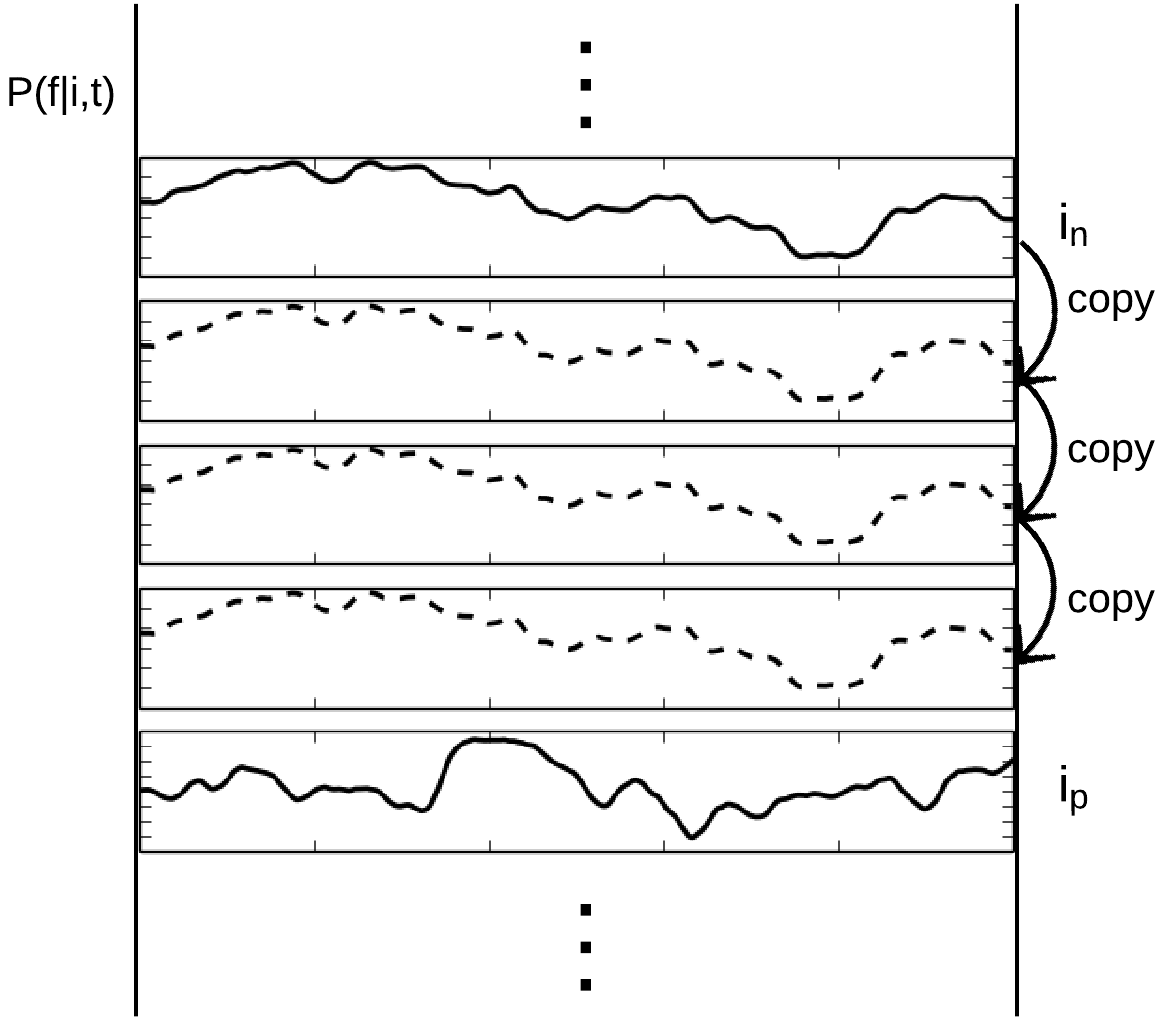
\includegraphics[width = \columnwidth]{figures/copy.png}

\vspace{2mm}
\emph{Schematic representation of the copy strategy.}
\end{center}

\begin{center}
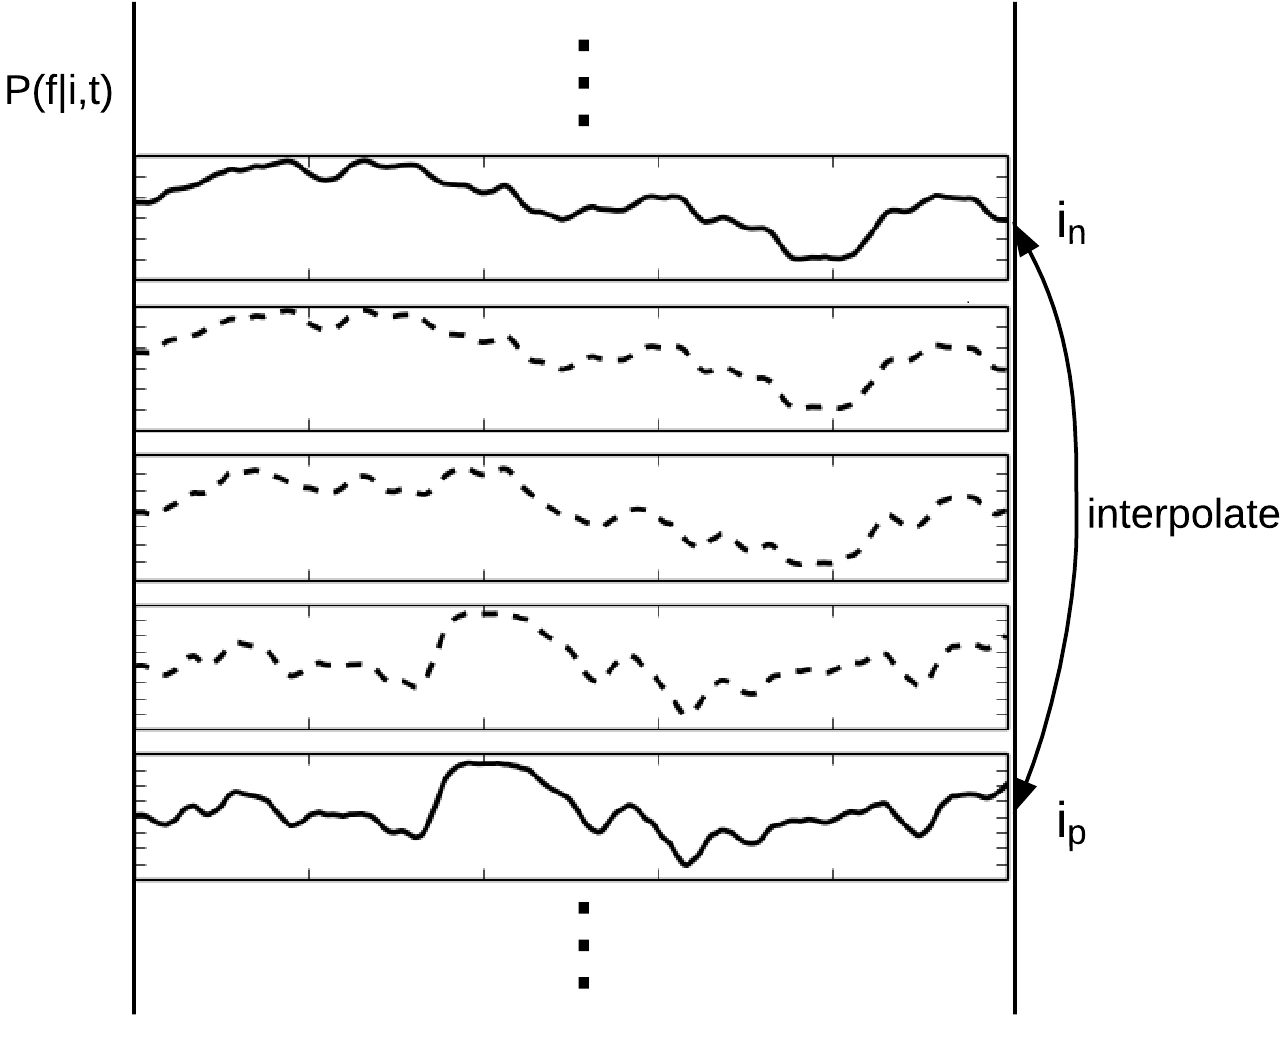
\includegraphics[width = \columnwidth]{figures/interpolate.png}

\vspace{2mm}
\emph{Schematic representation of the interpolate strategy.}
\end{center}

%$
%y_m(f,t)  = n_m(f,t) + \sum\limits_{s=0}^{S-1} y_{ms}(f,t)
%$
%
%$
%n_m(f,t) \sim \mathcal{N}_\mathbb{F}(0,\sigma_y^2)
%$
%
%$
%x_s(f,t) \sim \mathcal{N}_{\mathbb{F}}(0,\sigma_{x_s}^2(t))
%$

}

\headerbox{4. Convergence rate}{name=beta,column=2,row = 0}{
\sf

\textbf{Goal}: exploit the user input by controlling the convergence rate of the spectral envelopes when compared to other parameters of the model which are less well initialised.

\vspace{1mm}
\textbf{Idea}: convergence rate coefficient $\beta_{brake}(n)$ depends on the notes $n$:
$$
\beta_{brake}(n) = \left\{
\begin{array}{ll}
\beta_1, & \textrm{if }i_n\ \in \textrm{learning base} \\
\beta_0, & else
\end{array}
\right.,\  \beta_1 > \beta_0
$$
}

\headerbox{5. Results}{name=results,column=2,below=beta}{
\sf

\begin{center}
\begin{tabular}{ccccc}
\hline
\textbf{Options} & \textbf{Unsup.} & \multicolumn{3}{c}{\textbf{Semi-Guided}} \\\thickhline
& & Slope & Copy & Interp. \\\hline
NO & 67.68 & \textbf{68.38} & 65.00 & 43.68 \\
S & 73.91 & \textbf{75.07} & 71.44 & 52.07 \\
R & 66.46 & \textbf{68.28} & 64.13 & 47.05 \\
RS & 69.51 & \textbf{72.30} & 67.60 & 52.35 \\ \hline
B & 77.85 & \textbf{78.63} & 75.88 & 50.90 \\
SB & 74.64 & \textbf{76.54} & 72.47 & 45.68 \\
RB & 77.39 & \textbf{79.49} & 73.89 & 50.79 \\
RSB & 74.85 & \textbf{77.02} & 70.52 & 47.00 \\\thickhline
\end{tabular}


\vspace{2mm}
\emph{Mean F-Measure for the semi-guided and unsupervised approaches, considering the different initialisations of the non-annotated notes.}

\vspace{2mm}
\begin{tabular}{ccccc}
\hline
\textbf{} & \textbf{No brake} & \multicolumn{3}{c}{\textbf{Brake annotated notes}} \\\thickhline
& $\beta_{0,1}=0$ & $\beta_1=0.1$ & $\beta_1=1$ & $\beta_1=10$ \\\hline
B & \textbf{68,38} & 68,25 & 66,43 & 62,93 \\
SB & \textbf{75,07} & 74,84 & 74,29 & 72,74 \\
RB & 68,28 & 68,53 & \textbf{69,20} & 69,16 \\
RSB & 72,30 & 72,35 & 72,53 & \textbf{72,66} \\\thickhline
\end{tabular}

\vspace{0.1cm}
\begin{tabular}{ccccc}
\hline
\textbf{} & \textbf{Even} & \multicolumn{3}{c}{\textbf{Brake all notes}} \\\thickhline
& $\beta_{0,1}=10$ & $\beta_1=10.1$ & $\beta_1=11$ & $\beta_1=20$ \\\hline
B & 78,63 & 78,63 & \textbf{78,66} & \textbf{78,66} \\
SB & 76,54 & 76,54 & \textbf{76,55} & \textbf{76,55} \\
RB & 79,49 & 79,49 & 79,51 & \textbf{79,61} \\
RSB & 77,02 & 77,02 & \textbf{77,03} & 76,98 \\\thickhline
\end{tabular}

\vspace{2mm}
\emph{Mean F-Measure considering the different strategies for controlling the convergence rate of the annotated notes and the different options of the BHAD algorithm (priors).}
\end{center}
}

\headerbox{}{name=fig,column=3,row=0}{
\sf

\begin{center}

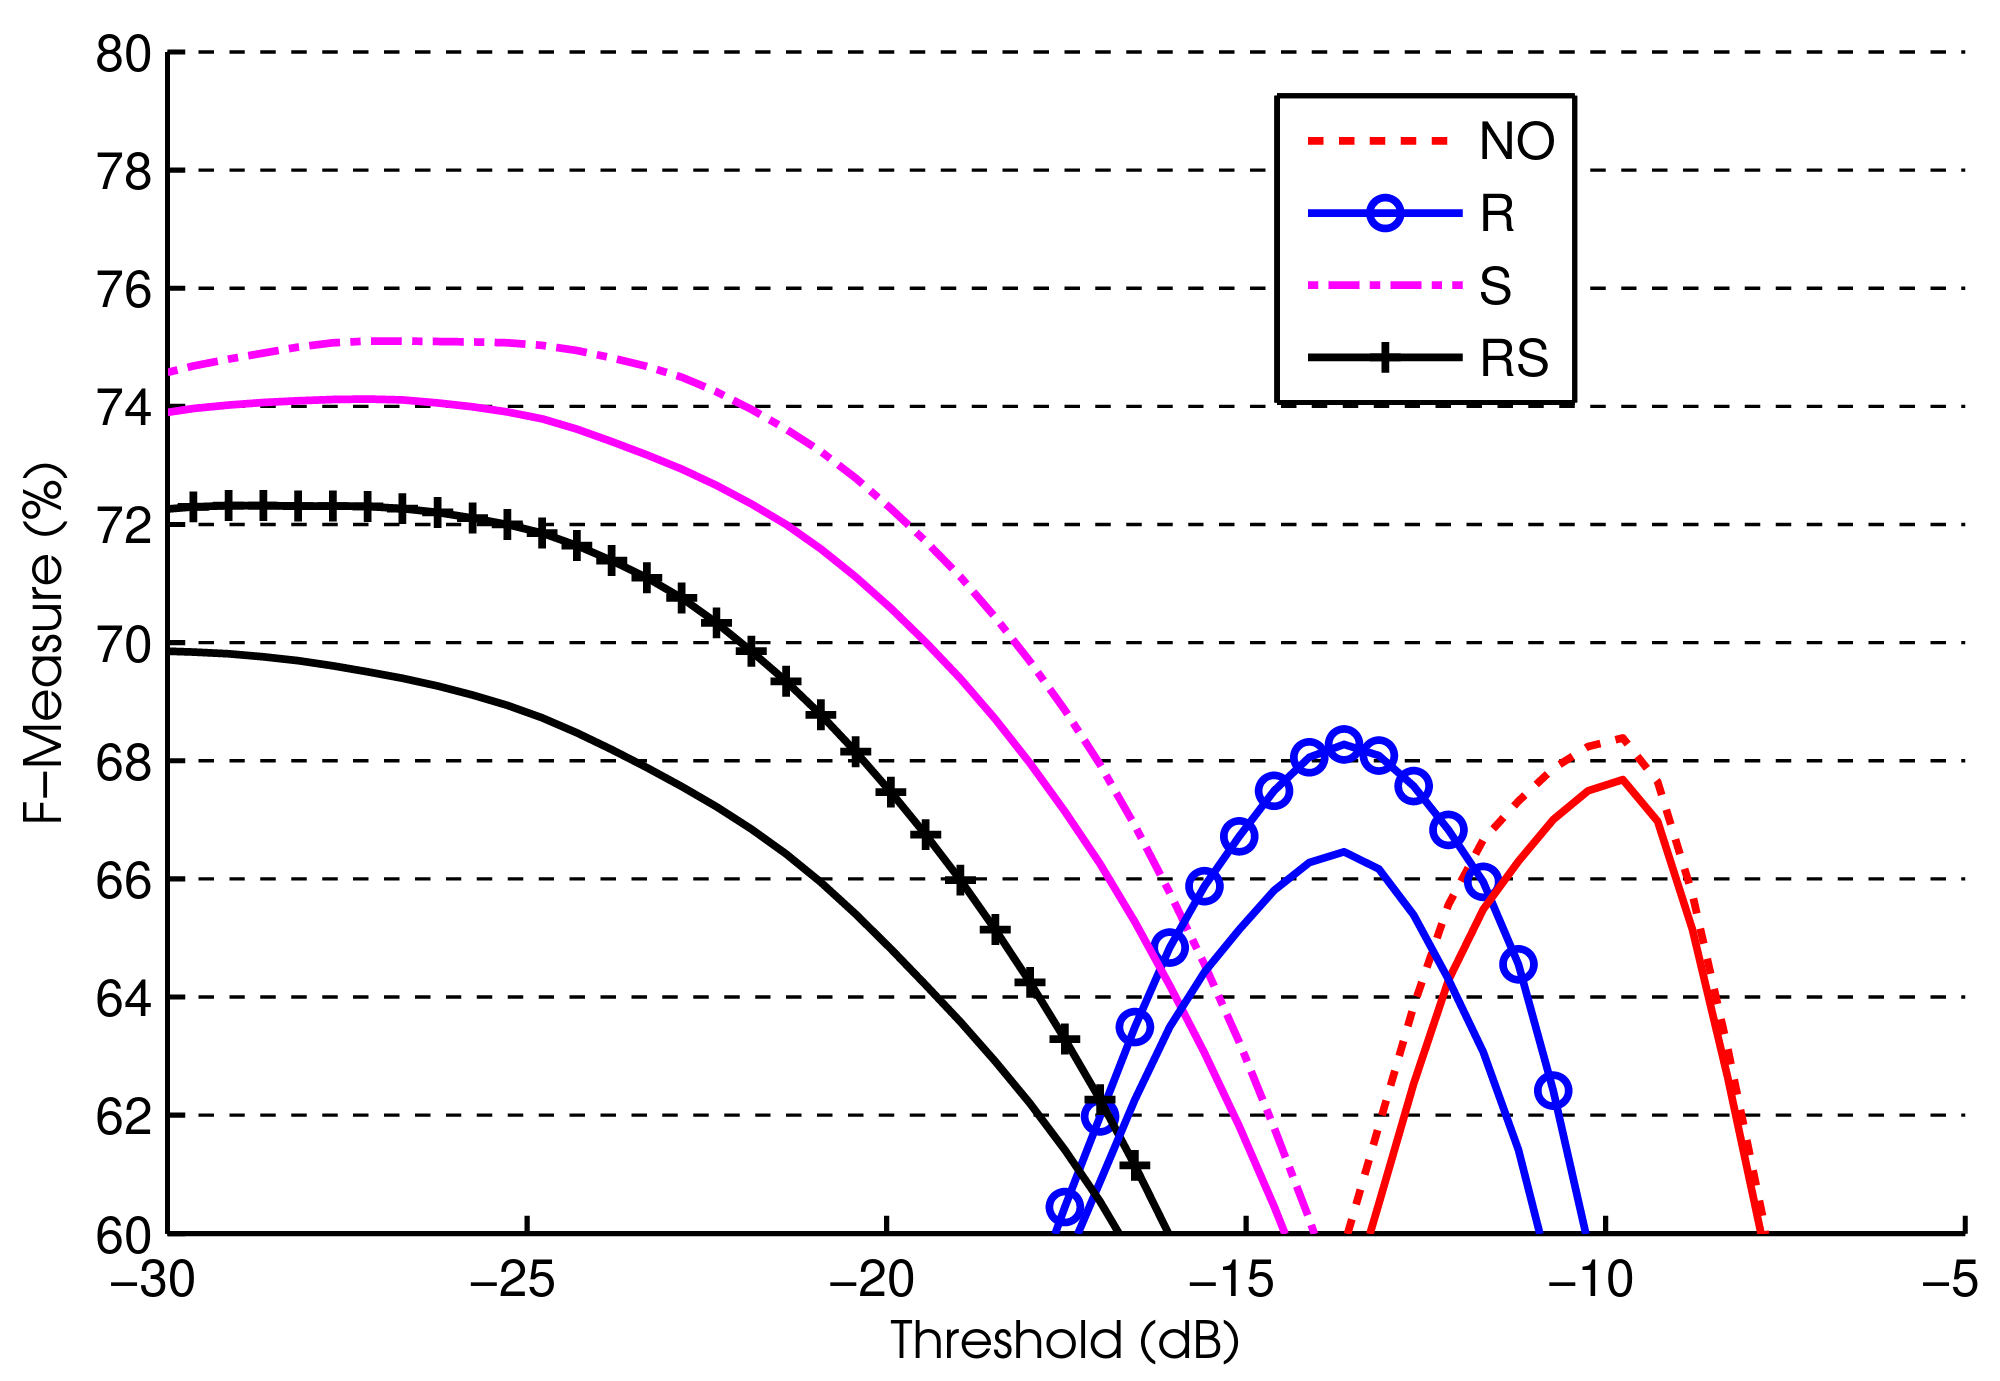
\includegraphics[width = \columnwidth]{figures/nobrake.png}

\vspace{3mm}
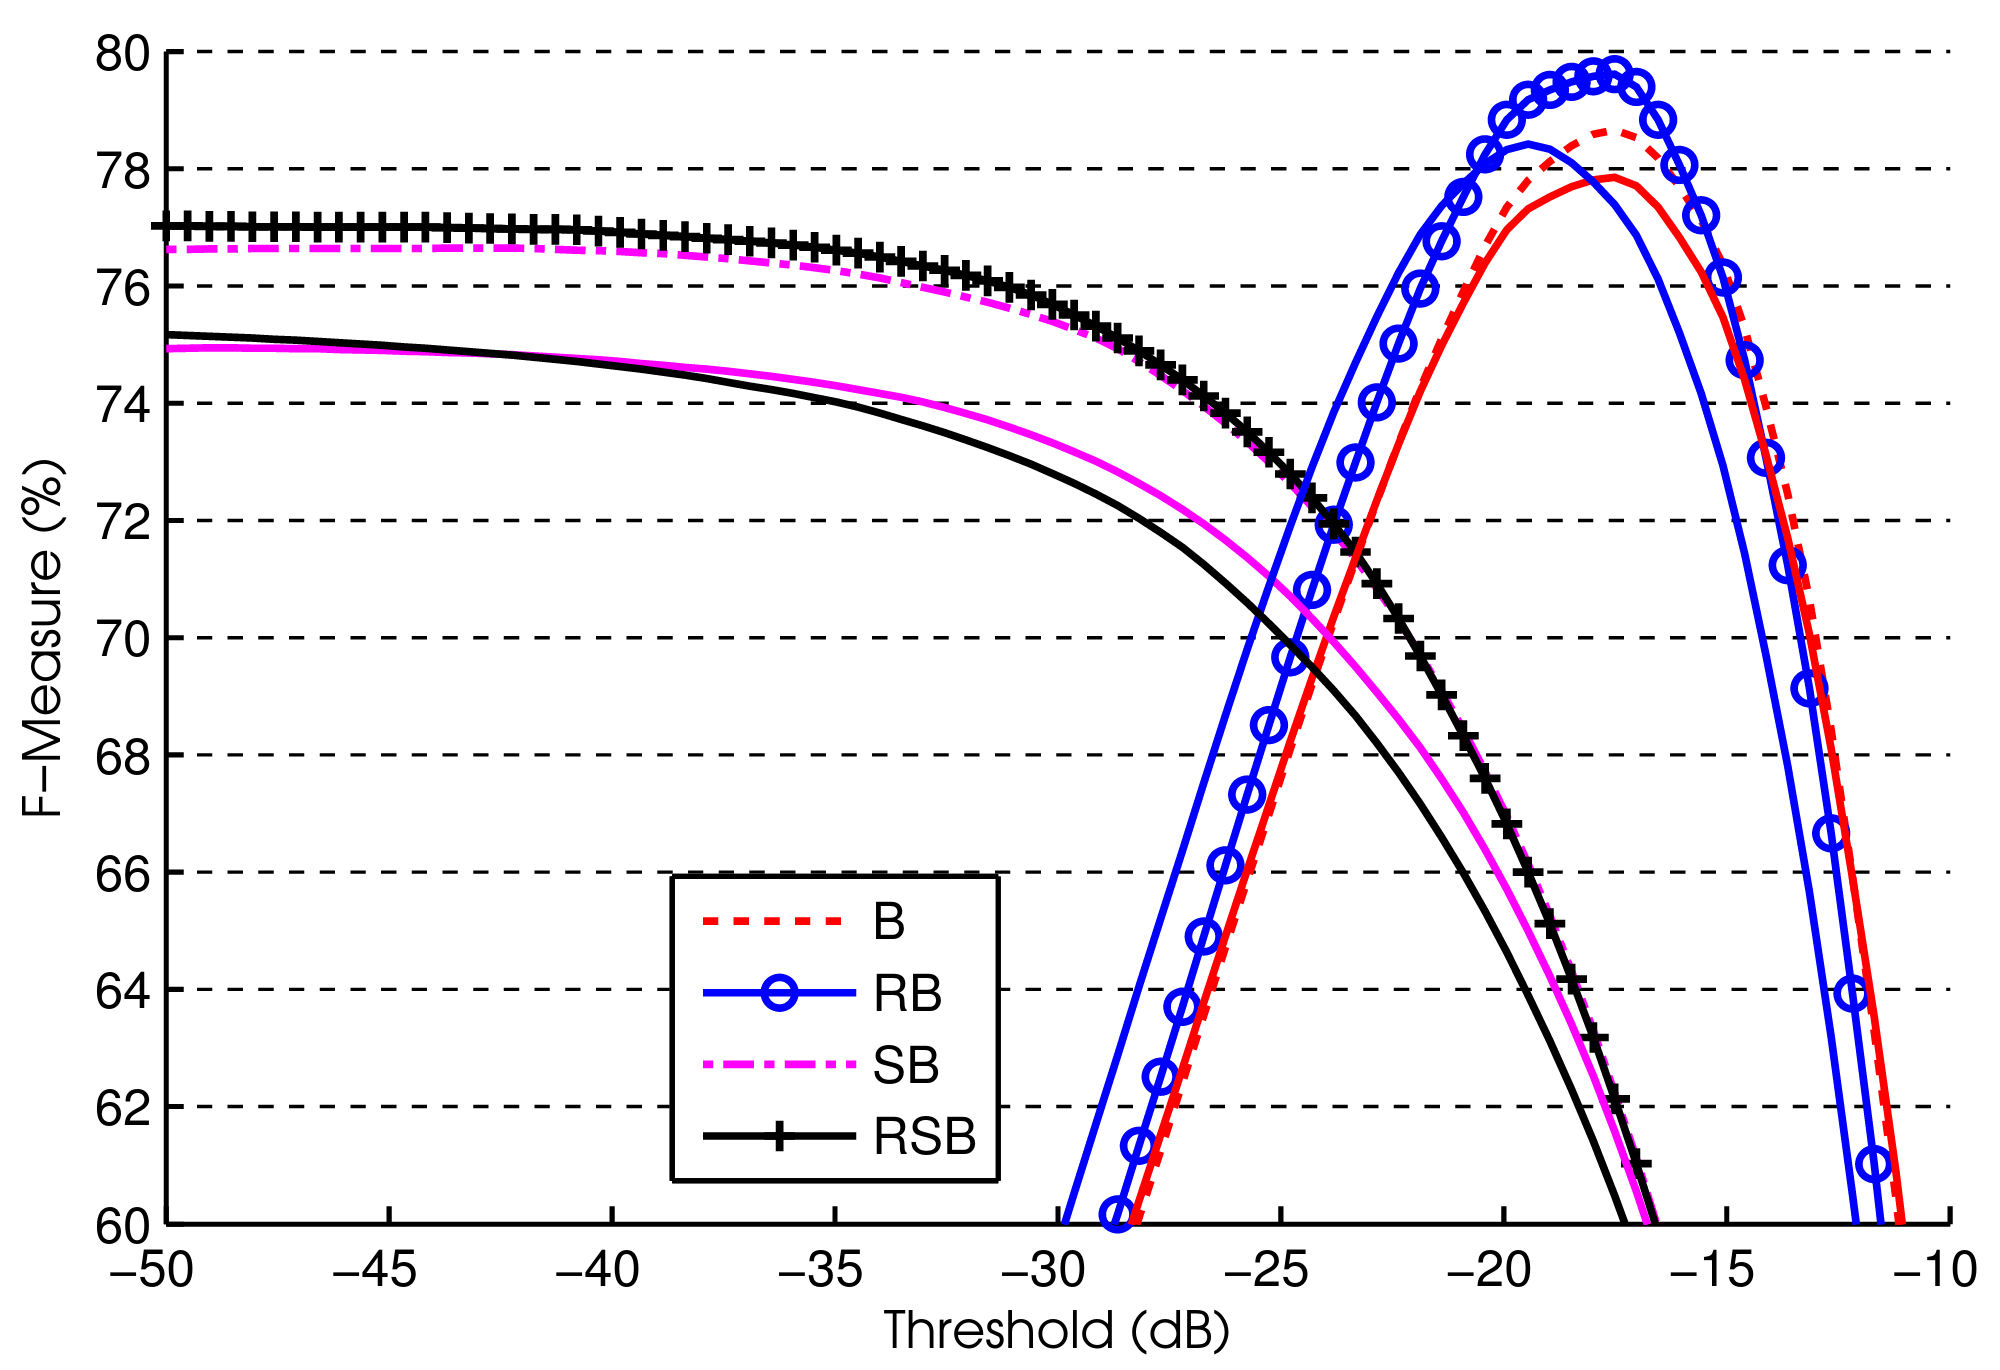
\includegraphics[width = \columnwidth]{figures/brake.png}\\
\emph{Results for the non-annotated notes (symbols) and the unsupervised approach without and with brake coefficients ($\beta_1=20$ and $\beta_0=10$).}
\end{center}
}

\headerbox{6. Conclusions}{name=conclus,column=3,below=fig}{
%\large
\sf
\textbf{Contributions:} \\
$\bullet$ Substantial gain in performance by using a learning step \\
$\bullet$ Better initialisation of the model parameters \\
\textbf{Future work:} \\
$\bullet$ Alternative strategies for the user annotation \\
$\bullet$ Involve the user in a more interative way

\vspace{1mm}
\footnotesize
\textbf{References:} \\
\mbox{[1]} B.Fuentes, R. Badeau \& G. Richard, "Blind harmonic adptive decomposition applied to supervised source separation", EUSIPCO~2012 \\
}

\end{poster}

\end{document}

